\documentclass[11pt,a4paper]{article}
\usepackage[margin=2.3cm]{geometry}
\usepackage{amsmath,amssymb,amsthm}
\usepackage{graphicx}
\usepackage{booktabs}
\usepackage[hidelinks]{hyperref}
\usepackage{caption}
\captionsetup{font=small,labelfont=bf}
\newtheorem{proposition}{Proposition}
\newtheorem{corollary}{Corollary}
\theoremstyle{remark}
\newtheorem*{remark}{Remark}
\newcommand{\rc}{r_c}
\newcommand{\Rb}{R_b}
\newcommand{\dd}{\mathrm{d}}

\title{The factor $u$ of the P18 profile:\\ a critically damped approach to the isothermal sphere,\\ and a burst experiment}
\author{B.~R. Parodi\\[2pt]\small companion note to \emph{From a primordial fluctuation to an idealised
rotation curve} (pf2irc), Sects.~2.1--2.3}
\date{1 November 2026}

\begin{document}
\maketitle

\begin{abstract}
\noindent The P18 profile is the singular isothermal sphere (SIS) multiplied by $u^2$,
with $u(x)=1+(x-1)e^{-x}$ and $x=R/\rc$. We show that $u$ is the unique solution of the
linear equation $u''+2u'+u=1$ with $u(0)=0$ and $u'(0)=2$: the approach of the profile
to the SIS is that of a \emph{critically damped} oscillator, with the radius in the role
of time and the core radius as damping length. The regular solutions form a
one-parameter family $u_b=1+(bx-1)e^{-x}$. For it we prove that the density crosses
that of the SIS at $x=1/b$, overshoots it if and only if $b>0$, and carries the mass
excess $c(b)=b^2/4+3b/2-3/2$, which is positive if and only if $b>\sqrt{15}-3$; P18 is
the member $b=1$, with $c=\tfrac14$, the only one whose damping length equals the core
radius defined by the central density. The non-singular isothermal sphere, by contrast,
approaches the SIS \emph{underdamped} in $\ln x$, as $x^{-1/2}\cos(\tfrac{\sqrt7}{2}\ln
x+\varphi)$, without a length scale. The double characteristic root has a simple reading:
two identical exponential relaxations in series. To test whether outflows from central
starbursts, decelerated by the infall, could produce such a single overshoot, we add to
the paper's self-similar collisionless shells a central baryonic mass that is repeatedly
blown out and falls back. The bursts flatten the cusp (density slope from $-2.5$ to
between $-0.8$ and $-1.8$) and rearrange the dark matter in a P18-like pattern, a rise,
a single peak and a zone of excess, but always on the scale of the accretion front, not
of the core, even when the gas is confined to two core radii. On nearly radial orbits
the displaced matter is deposited near its apocentres, where the infall turns it round;
an overshoot at the core would require the orbits there to become isotropic.
\end{abstract}

\tableofcontents
\bigskip

% =====================================================================
\section{The question}

In the paper the total matter of a late-type dwarf galaxy follows the P18 profile,
\begin{equation}
  \rho(R)=\frac{v^2u(x)^2}{4\pi GR^2}=\rho_{\rm SIS}(R)\,u(x)^2,\qquad
  u(x)=1+(x-1)\,e^{-x},\qquad x=\frac{R}{\rc},
  \label{eq:p18}
\end{equation}
with $\rho(0)=v^2/(\pi G\rc^2)$. All the information about the core is in the factor
$u$: for $u\equiv1$ the profile is the singular isothermal sphere (SIS). The form of
$u$ is empirical. This note asks two questions:
\begin{enumerate}
\item What is the mathematical structure of $u$? (Sects.~\ref{sec:ode}--\ref{sec:two})
\item Can a simple physical process, outflows from early central starbursts slowed down
  by the continuing infall, produce a deviation from the SIS of this kind?
  (Sect.~\ref{sec:runs})
\end{enumerate}
Throughout, $D\equiv\dd/\dd x$, $g\equiv u-1$, and $m(x)=\int_0^xu^2\,\dd x'$ is the
enclosed mass in units of $v^2\rc/G$.

% =====================================================================
\section{The differential equation}\label{sec:ode}

\begin{proposition}\label{prop:ode}
The function $u(x)=1+(x-1)e^{-x}$ is the unique solution on $[0,\infty)$ of
\begin{equation}
  u''+2u'+u=1,\qquad u(0)=0,\quad u'(0)=2 .
  \label{eq:ode}
\end{equation}
Equivalently, $g=u-1$ satisfies $(D+1)^2g=0$ with $g(0)=-1$, $g'(0)=2$.
\end{proposition}
\begin{proof}
With $g=(x-1)e^{-x}$ one finds $g'=(2-x)e^{-x}$ and $g''=(x-3)e^{-x}$, so
$g''+2g'+g=(x-3+4-2x+x-1)e^{-x}=0$; hence $u=1+g$ satisfies $u''+2u'+u=1$. Further
$u(0)=1-1=0$ and $u'(0)=g'(0)=2$. The equation is linear with constant coefficients, so
by the existence and uniqueness theorem for linear initial-value problems its solution
with given $u(0)$ and $u'(0)$ is unique.
\end{proof}

The characteristic polynomial of the homogeneous equation is $s^2+2s+1=(s+1)^2$, with
the double root $s=-1$. In the language of the damped oscillator,
$\ddot q+2\gamma\dot q+\omega_0^2q=0$ with $\gamma=\omega_0=1$: the damping is exactly
\emph{critical}. The variable $x$ plays the role of time, the deviation $g$ from the
isothermal value $u=1$ that of the displacement, and the core radius that of the
damping length.

\paragraph{The general solution and the regular family.} Every solution of
$u''+2u'+u=1$ has the form $u=1+(A+Bx)e^{-x}$. Since $\rho/\rho_{\rm SIS}=u^2$ and
$\rho_{\rm SIS}\propto x^{-2}$, the central density is finite if and only if $u(0)=0$,
i.e.\ $A=-1$. The \emph{regular} solutions therefore form the one-parameter family
\begin{equation}
  u_b(x)=1+(bx-1)\,e^{-x},\qquad u_b'(0)=b+1,
  \label{eq:family}
\end{equation}
and P18 is the member $b=1$.

\paragraph{Damping length and core radius.} If the equation is written for the
dimensional radius, $\lambda^2u''+2\lambda u'+u=1$ with derivatives with respect to
$R$, its solutions are $u_b(R/\lambda)$: $\lambda$ is the damping length. Near the
centre $u_b\simeq(b+1)R/\lambda$, so
$\rho(0)=v^2(b+1)^2/(4\pi G\lambda^2)$. Defining the core radius, as in the paper,
by $\rho(0)=v^2/(\pi G\rc^2)$ gives
\begin{equation}
  \rc=\frac{2\lambda}{b+1}.
\end{equation}
\begin{corollary}
P18 ($b=1$) is the only regular member whose damping length equals the core radius
defined by the central density.
\end{corollary}

% =====================================================================
\section{Properties of the regular family}\label{sec:props}

\begin{proposition}\label{prop:props}
For $u_b$ of Eq.~\eqref{eq:family}:
\begin{enumerate}
\item[(i)] \emph{Crossing.} For $b>0$, $u_b<1$ for $x<1/b$ and $u_b>1$ for $x>1/b$: the
  density crosses that of the SIS exactly at $x=1/b$. For $b\le0$, $u_b<1$ everywhere.
\item[(ii)] \emph{Overshoot.} $u_b$ exceeds 1 somewhere if and only if $b>0$; it then
  has a single maximum, $u_{\max}=1+b\,e^{-(b+1)/b}$ at $x=(b+1)/b$, and approaches 1
  monotonically beyond.
\item[(iii)] \emph{Mass excess.} $m(x)\to x+c(b)$ for $x\to\infty$, with
  \begin{equation}
    c(b)=\int_0^\infty(u_b^2-1)\,\dd x=\frac{b^2}{4}+\frac{3b}{2}-\frac32 ,
    \label{eq:cb}
  \end{equation}
  which is positive if and only if $b>\sqrt{15}-3\simeq0.873$.
\item[(iv)] \emph{Centre.} $u_b=(b+1)x-(b+\tfrac12)x^2+O(x^3)$, so
  $\rho/\rho(0)=1-\frac{2b+1}{b+1}\,x+O(x^2)$: the density falls linearly with radius
  unless $b=-\tfrac12$.
\end{enumerate}
\end{proposition}
\begin{proof}
(i) $u_b-1=(bx-1)e^{-x}$ has the sign of $bx-1$. (ii) For $b\le0$, $bx-1<0$ for all
$x\ge0$. For $b>0$, $u_b'=(b+1-bx)e^{-x}$ vanishes only at $x=(b+1)/b$, where $u_b$ is
maximal; inserting gives $u_{\max}$; beyond, $u_b'<0$ and $u_b\to1$. (iii) With
$g=(bx-1)e^{-x}$, $u^2-1=2g+g^2$, and with $\int_0^\infty x^ne^{-x}\dd x=n!$ and
$\int_0^\infty x^ne^{-2x}\dd x=n!/2^{n+1}$,
$\int_0^\infty2g\,\dd x=2(b-1)$ and
$\int_0^\infty g^2\,\dd x=b^2\cdot\tfrac14-2b\cdot\tfrac14+\tfrac12$. The sum is
Eq.~\eqref{eq:cb}. Its positive root is $b=-3+\sqrt{15}$. Since $m'=u^2\to1$ with an
exponentially small difference, $m(x)-x\to c(b)$. (iv) Expanding $e^{-x}=1-x+\tfrac12x^2
+O(x^3)$ in $1+(bx-1)e^{-x}$ gives the series, and
$\rho/\rho(0)=[u_b/((b+1)x)]^2$.
\end{proof}

For P18 ($b=1$): the density crosses the SIS at $x=1$, i.e.\ at $R=\rc$; the maximum
is $u=1+e^{-2}=1.135$ at $x=2$ ($u^2=1.289$); the mass excess is $c=\tfrac14$; and
$\rho/\rho(0)=1-\tfrac32x+\dots$ near the centre (Fig.~\ref{fig:family}a). The two
properties are distinct: an overshoot exists for every $b>0$, but a positive mass excess
needs $b>0.873$, since the deficit inside the crossing must be outweighed by the excess
outside it.

\paragraph{The displaced mass.} Define $F(x)=x-m(x)$, the mass that P18 lacks inside
$x$ compared with the SIS. Since $m'=u^2$,
\begin{equation}
  u^2=1-F'(x):
  \label{eq:flux}
\end{equation}
$F$ is the mass carried outward through the sphere of radius $x$, relative to the SIS.
For P18, $F(0)=0$, $F$ is maximal where $u=1$, at $x=1$, with $F(1)=1-m(1)=0.520$;
it vanishes at $x=3.29$ and tends to $-c=-0.25$. So $0.520\,v^2\rc/G$ is taken out of
the core and $\int_1^\infty(u^2-1)\,\dd x=c+1-m(1)=0.770\,v^2\rc/G$ is added outside
it. (Numbers: \texttt{ode\_checks.py}.)

% =====================================================================
\section{Comparison with the isothermal sphere}\label{sec:emden}

A fully thermalised self-gravitating gas, the non-singular isothermal sphere, also has
a finite central density and tends to the SIS. With $\rho=\rho_0e^{-\psi}$ and
$\xi=R/r_0$, $r_0^2=\sigma^2/(4\pi G\rho_0)$, it obeys
\begin{equation}
  \psi''+\frac2\xi\,\psi'=e^{-\psi},\qquad \psi(0)=\psi'(0)=0,
\end{equation}
whose singular solution $e^{-\psi_s}=2/\xi^2$ is the SIS. Writing $\psi=\psi_s+\delta$
and linearising, $e^{-\psi}\simeq(2/\xi^2)(1-\delta)$, so
$\delta''+(2/\xi)\delta'+(2/\xi^2)\delta=0$. In the variable $s=\ln\xi$ this is
\begin{equation}
  \delta_{ss}+\delta_s+2\delta=0,\qquad\text{roots }s=-\tfrac12\pm\tfrac{\sqrt7}{2}\,i,
\end{equation}
so that $\rho/\rho_{\rm SIS}-1=-\delta\propto\xi^{-1/2}\cos(\tfrac{\sqrt7}{2}\ln\xi+
\varphi)$. The isothermal sphere approaches the SIS \emph{underdamped in} $\ln R$: its
density oscillates about the SIS without end, with decreasing amplitude and no length
scale. For the same central density ($\rc=\sqrt8\,r_0$) its first maximum is
$\rho/\rho_{\rm SIS}=1.66$ at $x=1.44$ and its first minimum 0.83 at $x=13$
(Fig.~\ref{fig:family}b). P18 approaches the SIS \emph{critically damped in} $R$, with
a single overshoot and the damping length $\rc$. A mechanism for P18 must therefore
carry its own length scale; plain thermalisation, the classic idea behind isothermal
cores, would give the scale-free ringing of the isothermal sphere.

\begin{figure}[t]
\centering
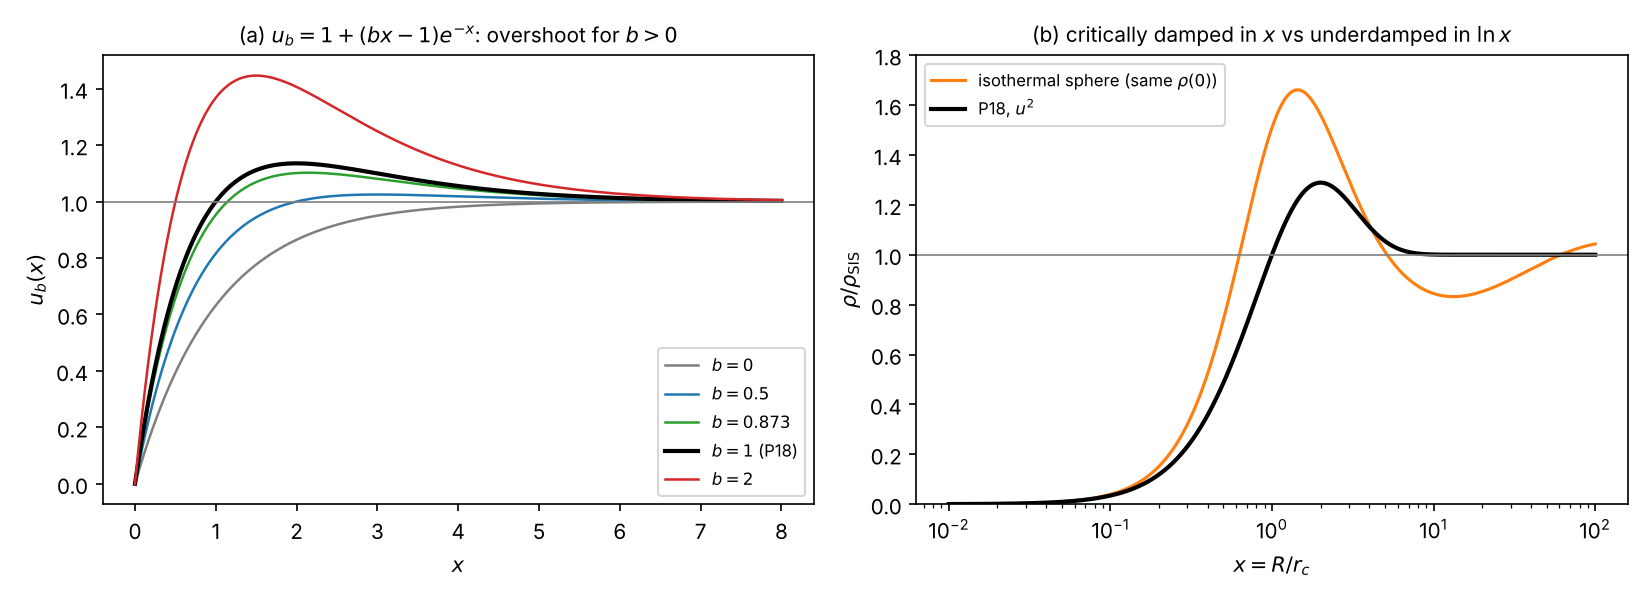
\includegraphics[width=\textwidth]{fig_ufamily.png}
\caption{(a) The regular family $u_b=1+(bx-1)e^{-x}$: an overshoot for every $b>0$, a
positive mass excess for $b>0.873$, P18 at $b=1$. (b) Density relative to the SIS for
P18 (black) and for the non-singular isothermal sphere with the same central density
(orange): one critically damped overshoot against an underdamped oscillation in $\ln
x$. Script: \texttt{fig\_ufamily.py}.}
\label{fig:family}
\end{figure}

% =====================================================================
\section{A two-stage reading}\label{sec:two}

The double root has a simple interpretation. Write $(D+1)^2g=0$ as the chain
\begin{equation}
  (D+1)\,Q=0,\qquad (D+1)\,g=Q .
\end{equation}
The first gives $Q=Q_0e^{-x}$: a quantity $Q$ relaxes exponentially with the length
$\rc$. The second says that $g$ relaxes, with the same length, towards the value that
$Q$ imposes; its solution is $g=(g_0+Q_0x)\,e^{-x}$, the factor $x$ coming from the
resonance of the two equal rates. For P18, $g_0=-1$ and $Q_0=1$. Critical damping is
thus equivalent to two identical first-order relaxations in series, like two
compartments with equal rate constants; unequal lengths $\lambda_1\ne\lambda_2$ would
give a sum of two exponentials (overdamping), and an oscillatory coupling would give
ringing.

\begin{remark}
This is a reformulation, not a derivation. A physical theory of $u$ would have to name
the two processes, explain why they share the length $\rc$ and why the central
conditions select $b=1$. Nothing in this note does so.
\end{remark}

% =====================================================================
\section{A burst experiment}\label{sec:runs}

\subsection{The idea and the model}
One physical reading of a single damped overshoot is an outflow slowed down by the
infall: early central starbursts blow gas out, and the continuing accretion stops it.
Dark matter is collisionless and feels the gas only through gravity, so the test must
ask whether repeated changes of the central baryonic potential rearrange the dark
matter in the P18 pattern: a deficit inside $\rc$, a single excess just outside it.

We use the one-dimensional collisionless shells of the paper (its Appendix~H; units
$G=v=1$): 2000 shells with masses spaced logarithmically from $10^{-4}$ to 1, each
following its cycloid with $E=-\tfrac12$ until turnaround, where it receives
$j=\sqrt2\lambda R_{\rm ta}$ ($\lambda=0.035$), and afterwards
\begin{equation}
  \ddot r=-\frac{M_{\rm enc}(r)}{r^2}+\frac{j^2}{r^3}
  -\frac{M_b(t)\,r}{[r^2+a(t)^2]^{3/2}} ,
\end{equation}
with a softening $2\times10^{-4}t$, leapfrog integration with an adaptive global step,
and shells free to cross. The last term is a prescribed central baryonic mass, a
Plummer sphere of mass $M_b=f_b\,\xi_f\,t$ (a fraction $f_b$ of the mass inside the
front, $\xi_f=0.2$) and radius $a(t)$ that jumps between a compact value $a_c\,t$
($a_c=0.002$, about a third of the model's core) and an expanded value $a_e\,t$. A cycle
lasts $P\,t$ (uniformly spaced in $\ln t$), compact for half of it. All scales grow as
$t$, so the runs stay self-similar. We stack 16 snapshots between 0.7 and 1 times the
turnaround time of the outermost shell and use $\xi=R/vt$; the front is at
$\xi\simeq0.21$ and the paper's core at about $\xi_b/y\simeq0.006$. The run without
baryons is the reference.

\paragraph{Diagnostics.} (a) The logarithmic slope of the dark-matter density at
$\xi=0.002$--0.006. (b) The displaced dark matter,
$F(\xi)=M_{\rm ref}(<\xi)-M_{\rm run}(<\xi)$ (per unit $t$), the analogue of
$x-m(x)$ for P18: positive where dark matter has been removed, negative where it has
accumulated. The noise of $F$, estimated from the even minus the odd snapshots of the
reference run, is at most $1.2\times10^{-3}$.

\subsection{Results}
\begin{table}[h]
\centering\small
\caption{The runs ($f_b$: baryonic mass fraction; $a_e$: expanded radius; $P$: cycle
length in units of $t$). Slope: dark-matter density at $\xi=0.002$--0.006. $F$:
displaced dark matter, its peak and the radius beyond which it turns negative
(accumulation). Template rms: residual of the best fit of $A\,(x-m(x))$, $x=\xi/\xi_s$,
in units of the peak, over $\xi=0.003$--1.}
\label{tab:runs}
\begin{tabular}{lccccccc}
\toprule
run & $f_b$ & $a_e$ & $P$ & slope & peak of $F$ (at $\xi$) & $F<0$ beyond & rms\\
\midrule
reference & 0 & -- & -- & $-2.46$ & -- & -- & --\\
fb05 & 0.05 & 0.05 & 0.05 & $-1.28$ & 0.042 (0.20) & -- & 0.15\\
fb10 & 0.10 & 0.05 & 0.05 & $-0.77$ & 0.069 (0.22) & -- & 0.13\\
fb20 & 0.20 & 0.05 & 0.05 & $-1.26$ & 0.086 (0.22) & -- & 0.14\\
fb05fast & 0.05 & 0.05 & 0.01 & $-1.02$ & 0.051 (0.20) & -- & 0.16\\
fb10far & 0.10 & 0.20 & 0.05 & $-1.44$ & 0.072 (0.22) & -- & 0.12\\
fb05ae02 & 0.05 & 0.02 & 0.05 & $-1.17$ & 0.035 (0.22) & 0.61 & 0.16\\
fb05ae01 & 0.05 & 0.01 & 0.05 & $-1.80$ & 0.020 (0.20) & 0.48 & 0.19\\
fb02ae01 & 0.02 & 0.01 & 0.05 & $-2.27$ & 0.006 (0.09)$^a$ & 0.28$^a$ & 0.26\\
\bottomrule
\end{tabular}

\smallskip
\footnotesize $^a$ Only 3--5 times the noise.
\end{table}

\begin{figure}[t]
\centering
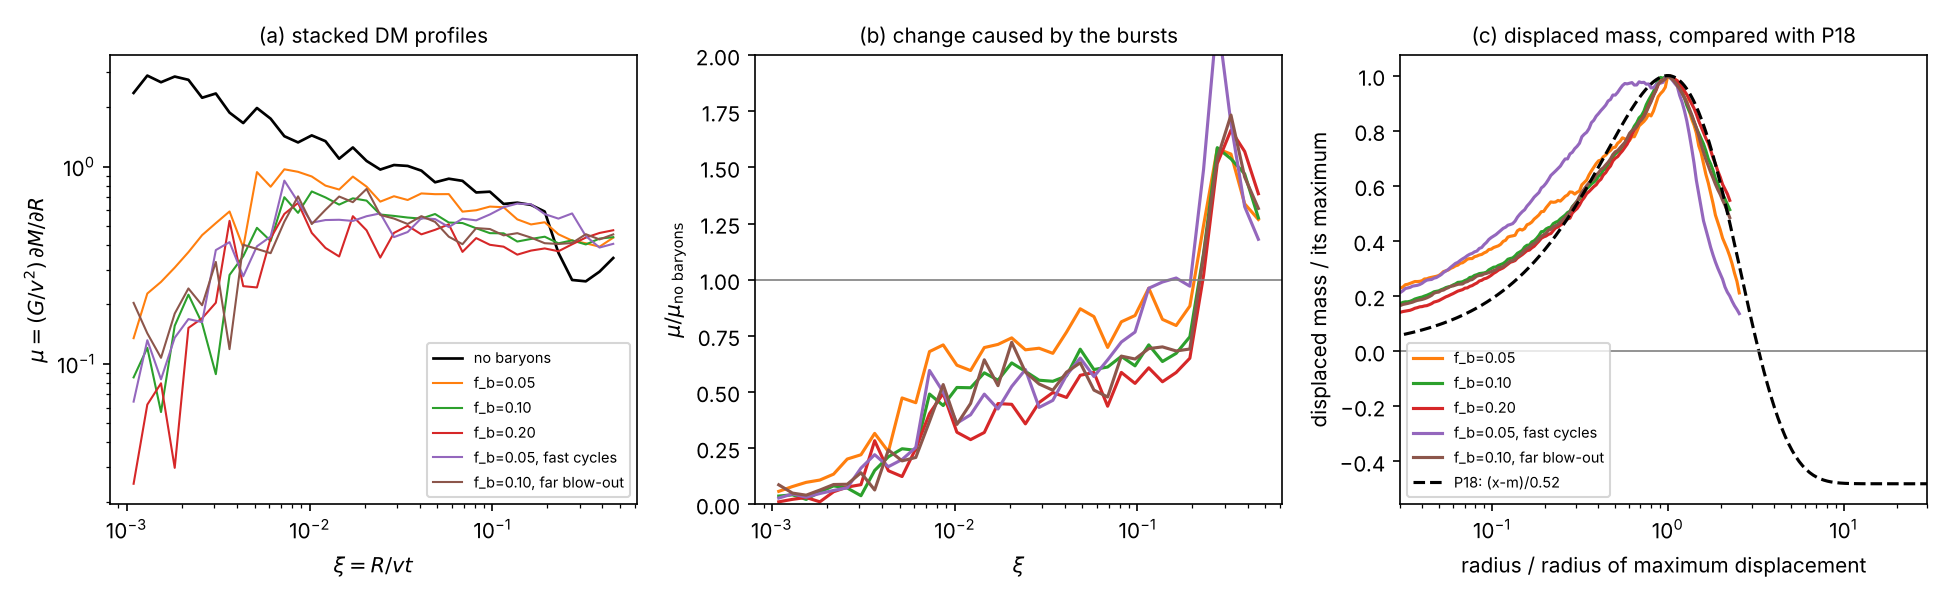
\includegraphics[width=\textwidth]{fbshells.png}
\caption{The first six runs. (a) Stacked dark-matter profiles, $\mu=(G/v^2)\,\partial
M/\partial R$ against $\xi=R/vt$. (b) Ratio to the reference run: the dark matter is
reduced at all radii inside the front and piles up just beyond it. (c) Displaced
dark matter scaled to its peak, against radius scaled to the radius of the peak,
compared with $(x-m)/0.52$ of P18. Script: \texttt{fig.py}.}
\label{fig:runs1}
\end{figure}

\begin{figure}[t]
\centering
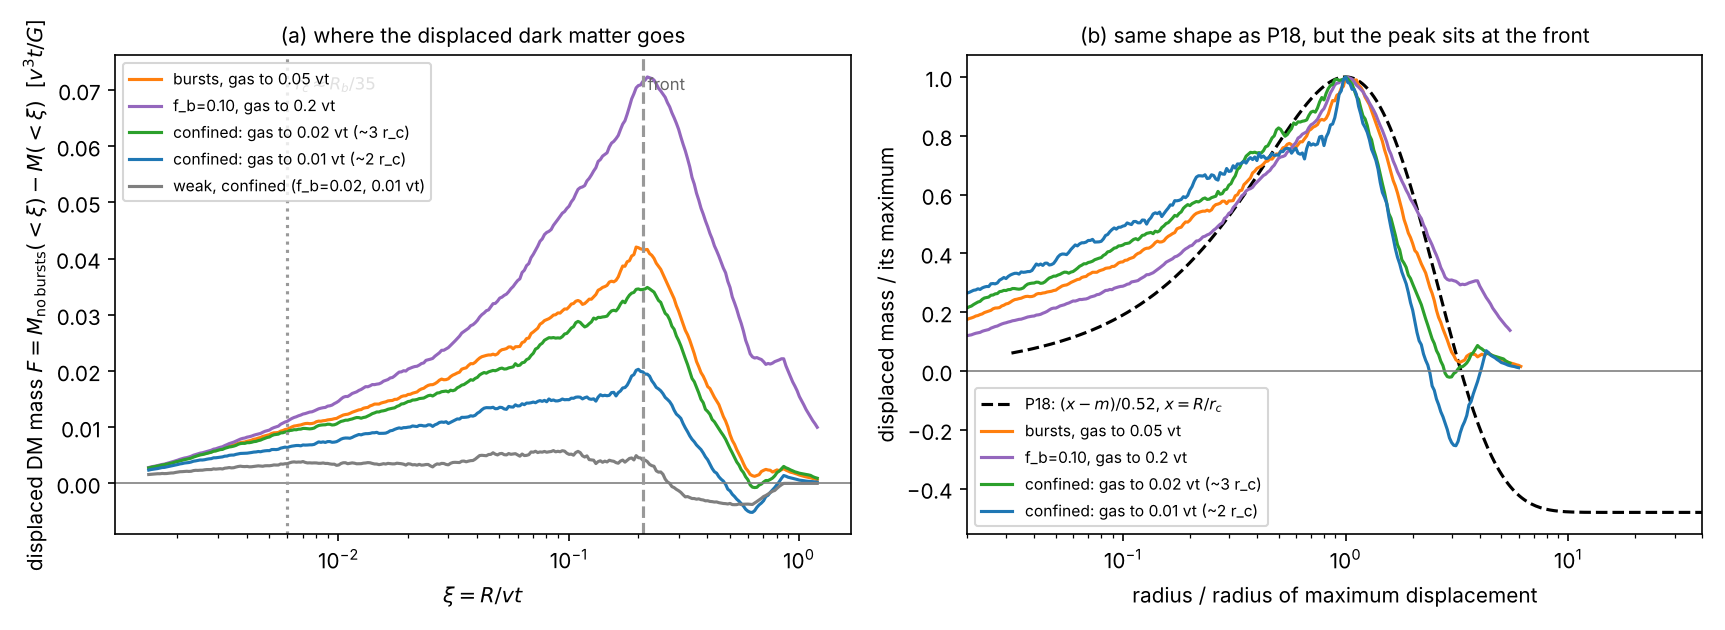
\includegraphics[width=\textwidth]{fbshells2.png}
\caption{(a) Displaced dark matter for five runs, including the three with the gas
confined to 0.01--0.02\,$vt$, about 2--3 core radii; dotted: the model's core, dashed:
the front. (b) The same, scaled to the peak, with P18. Script: \texttt{fig2.py}.}
\label{fig:runs2}
\end{figure}

\begin{enumerate}
\item \emph{The bursts flatten the cusp.} The inner slope rises from $-2.46$ to between
  $-0.8$ and $-1.8$ (Table~\ref{tab:runs}): repeated changes of the central potential
  raise the energy of the central dark matter, as required for the settling into a
  core and as found in hydrodynamical simulations (e.g.\ \cite{PG12}). Weak confined
  bursts ($f_b=0.02$) barely change the slope.
\item \emph{The rearrangement has the P18 shape.} Scaled to its peak, the displaced
  mass rises, peaks and falls like $x-m(x)$ (Figs.~\ref{fig:runs1}c,
  \ref{fig:runs2}b); with the gas confined, it even turns negative at 2.4--2.8 times
  the radius of the peak (P18: 3.3), a single zone of accumulation without ringing.
  The P18 template fits with a residual of 12--19\% of the peak; a template without
  accumulation ($\arctan x$, the pseudo-isothermal sphere) fits worse in all runs but\n  fb20, where the two are equal (14--28\%).
\item \emph{But on the wrong scale.} The peak lies at the front, $\xi\simeq0.20$--0.22,
  about $35\,\rc$, in every run with a clear signal, and the accumulation lies beyond
  the front. Confining the gas to two or three core radii weakens the effect but does
  not move the peak inward (Fig.~\ref{fig:runs2}a). Inside the front the dark matter
  is reduced by 20--65\% at all radii, so the flat curve is lost.
\end{enumerate}

\subsection{Why the matter goes to the front}
In this one-dimensional model the dark matter moves on nearly radial orbits, which
spend most of their time near their apocentres. A burst raises a particle's energy and
moves its apocentre outward; the matter reappears far out, where the infall turns it
round, i.e.\ at the front. Depositing it at about $2\rc$ would require orbits that spend
their time near $\rc$, i.e.\ nearly isotropic orbits in the core. This is exactly the
second requirement for the settling into a core found in the companion note
\emph{Halting and settling}: an energy lift \emph{and} isotropy. The bursts supply the
first, not the second. In three dimensions the second could come from the radial-orbit
instability or a triaxial centre, which a spherical shell code cannot represent.

\paragraph{Caveats.} The baryons are prescribed, not evolved, and switch instantly; the
dark matter is spherical and one-dimensional; the cycling gas, 2--20\% of the galaxy's
mass, exceeds the 1.7\% of baryons that the dwarfs keep today; and the reference run is
a cusp, not P18. The results are indicative of a mechanism, not a model of real dwarfs.

% =====================================================================
\section{Conclusions}
\begin{enumerate}
\item The factor $u$ of P18 is the unique solution of $u''+2u'+u=1$, $u(0)=0$,
  $u'(0)=2$: a critically damped approach to the isothermal value, with the core radius
  as damping length (Proposition~\ref{prop:ode}).
\item The regular solutions form the family $u_b=1+(bx-1)e^{-x}$. A single overshoot
  exists for $b>0$; a positive mass excess, $c(b)=b^2/4+3b/2-3/2$, for $b>0.873$. P18
  is $b=1$, $c=\tfrac14$, the member whose damping length equals the core radius
  (Proposition~\ref{prop:props}). Its density falls linearly at the centre.
\item The isothermal sphere approaches the SIS underdamped in $\ln R$, without a length
  scale; P18 critically damped in $R$, with the scale $\rc$.
\item Critical damping is equivalent to two identical exponential relaxations in
  series; their physical identity is open.
\item Bursts of central gas flatten the cusp and rearrange the dark matter in a P18-like
  pattern, but on the scale of the front, not the core. A single overshoot at about
  $2\rc$ needs, in addition to the energy, isotropic orbits in the core.
\end{enumerate}

\begin{thebibliography}{9}
\bibitem{PG12} Pontzen, A., \& Governato, F. 2012, MNRAS, 421, 3464
\end{thebibliography}

\section*{Files in this package}
\begin{small}
\begin{tabular}{@{}lp{0.62\textwidth}@{}}
\texttt{ode\_checks.py} & numerical checks of Sects.~2--4; output \texttt{ode\_checks\_out.txt}\\
\texttt{fig\_ufamily.py} & Fig.~1\\
\texttt{p18core.py} & P18 functions $u$, $m$ (series near the centre)\\
\texttt{fbshells.py} & the shell code with the central baryonic component\\
\texttt{runall.py} & the nine runs (\texttt{python3 runall.py [names]}); logs \texttt{runs.log}, \texttt{runs2.log}\\
\texttt{run\_*.pkl} & the stacked snapshots of the runs\\
\texttt{analyse.py}, \texttt{analyse2.py} & slopes, displaced mass, template fits; outputs \texttt{analyse\_out.txt}, \texttt{analyse2\_out.txt}\\
\texttt{fig.py}, \texttt{fig2.py} & Figs.~2 and 3 (run \texttt{analyse.py} on the first six runs before \texttt{fig.py})\\
\end{tabular}
\end{small}

\end{document}
